\begin{block}{Study Area \& Variable Definitions}
    \begin{figure}
        \centering
        \caption{Composite anomalies of \SI{500}{\hecto\pascal} geopotential height (color) and precipitable water (contours) from 4 days preceding regional intense precipitation days in the Ohio River Basin to one day following.}
        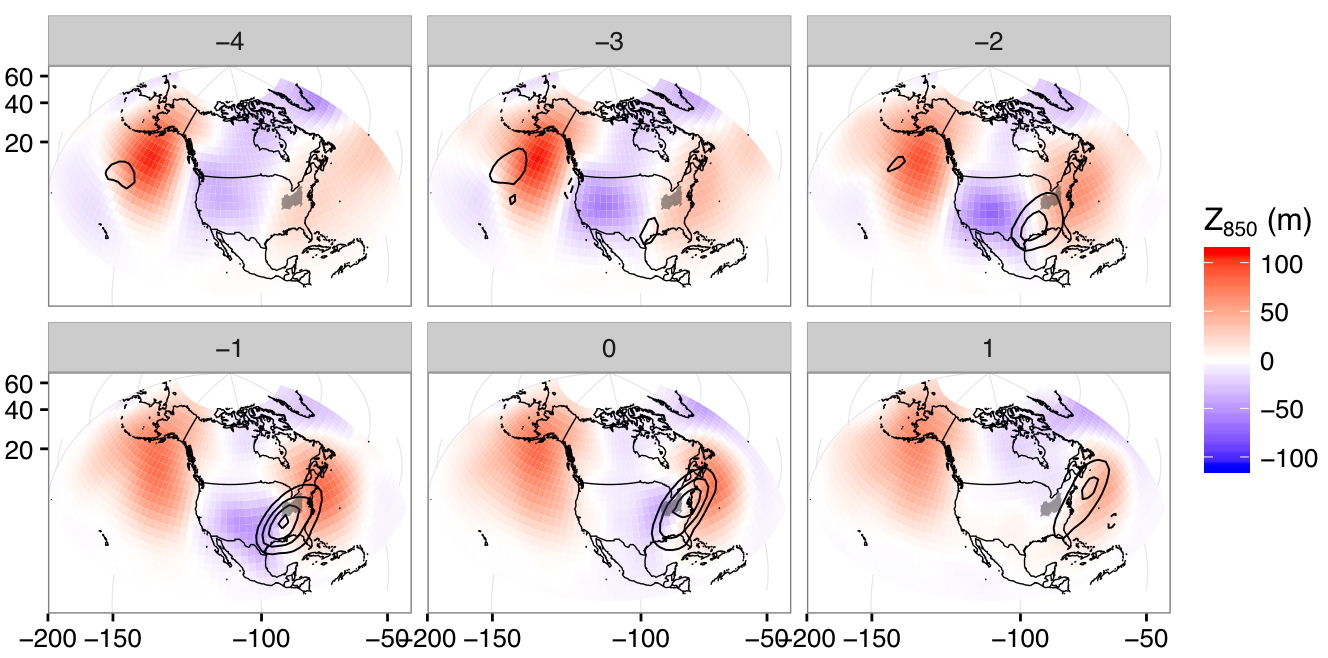
\includegraphics[width=\columnwidth]{../FigExternal/djf_composites}
        \label{fig:djf-composites}
    \end{figure}
    Study \cite{Farnham2016} of regional intense precipitation events in the Ohio River Basin (\cref{fig:djf-composites}) reveals the dominance of a ridge (somtimes stationary, sometimes transient) over the Western Atlantic and a transient cyclone propagating eastward.
    Following our conceptual framing (\cref{fig:apr2011}) we define the following variables, separated into planetary-scale and synoptic-scale.
    \begin{description}
        \item[Moisture] the daily net moisture flux into the green box in \cref{fig:study-area}
        \item[Planetary] the monthly AMO and daily NAO indices from the CPC
         \item[Synoptic] Mean SST anomaly over the Gulf of Mexico (\cref{fig:study-area}); the geopotential height anomaly over West Atlantic Ridge (\cref{fig:study-area}); and a one-dimensional index, based on local regression \cite{Loader1999} relating cyclone position (2D) to expected moisture flux; see \cref{fig:track-given-flux}
    \end{description}
    \begin{figure}
        \centering
        \includegraphics[width=0.8\columnwidth]{map_inset}
        \caption{Study Area. Shaded area shows the Ohio River Basin.}
        \label{fig:study-area}
    \end{figure}
\end{block}
